\documentclass[a4paper]{article}
\usepackage[utf8]{inputenc}   % pro unicode UTF-8
\usepackage[czech]{babel} %jazyk dokumentu
\usepackage{listings}
\usepackage{color}
\usepackage[T1]{fontenc}
\usepackage{amssymb}
\usepackage{hyperref}
\usepackage{listingsutf8}
\usepackage{graphicx}
\usepackage{amsmath}
\usepackage[margin={1cm,2cm}]{geometry}

\graphicspath{ {/} }

\def\doubleunderline#1{\underline{\underline{#1}}}

%%%%%%%%%%%%%%%%%%%%%%%%%%%%%%%%%%%%%%%%%%%%%%%%%%%%%%%%%%%%%

\begin{document}

\noindent
\textbf{Predmet: Vyrokova a predikatorova logika}\\
\textbf{Ukol: 3.}\\
\textbf{Verze: 1.}\\
\textbf{Autor: David Napravnik}

\section*{$S \subseteq T \Rightarrow \Theta(T) \subseteq \Theta(S)$}
Neplati.\\
Podle tvrzeni kde pro kazde dve teorie $T$ a $T'$ plati $T \subseteq T' \Rightarrow \Theta^{\mathbb{P}}(T) \subseteq \Theta^{\mathbb{P}}(T')$\\
Spravna implikace by tedy mela byt: $S \subseteq T \Rightarrow \Theta(S) \subseteq \Theta(T)$


\section*{$\Theta(S \cup T) = \Theta(S) \cup \Theta(T)$}
Plati, mnoziny jsou ekvivalentni, viz obrazek s mnozinami.


\section*{$\Theta(S \cap T) = \Theta(S) \cap \Theta(T)$}
Plati, mnoziny jsou ekvivalentni, viz obrazek s mnozinami.


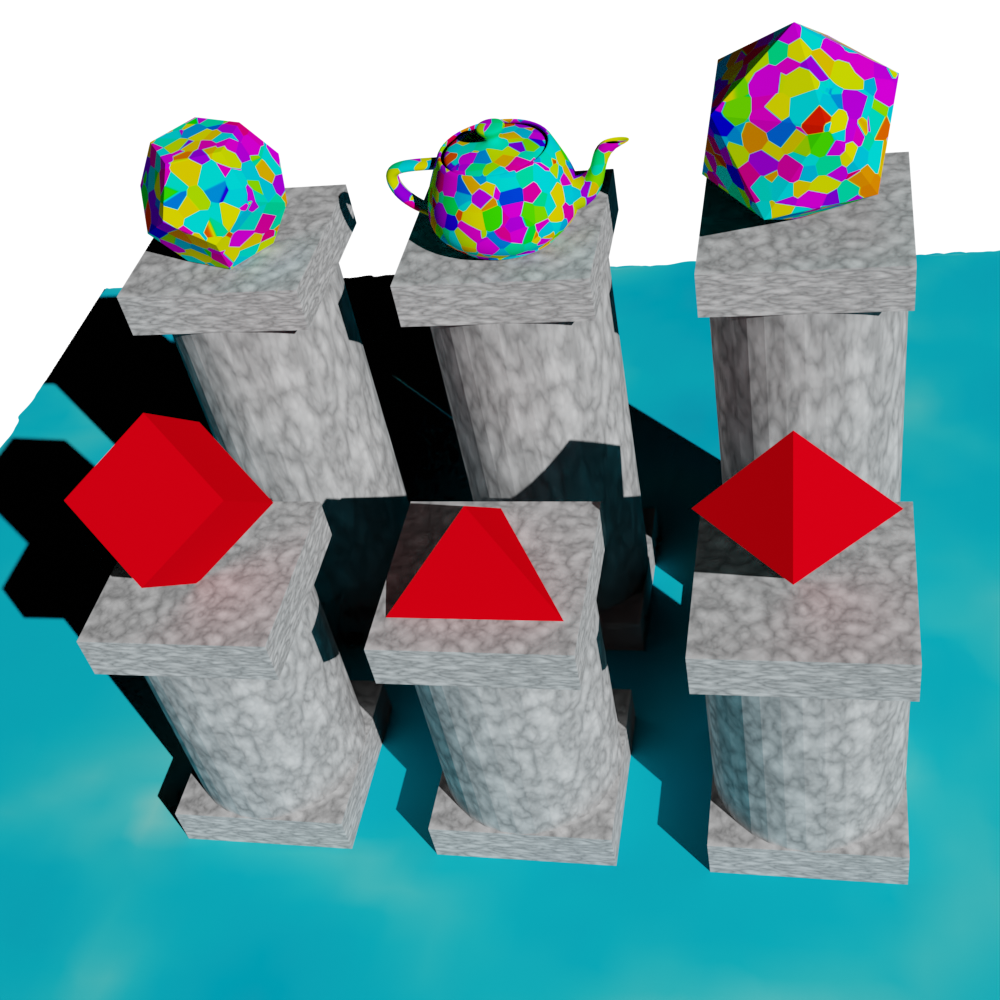
\includegraphics[width=\textwidth]{hw3.png}






\end{document}